% Options for packages loaded elsewhere
% Options for packages loaded elsewhere
\PassOptionsToPackage{unicode}{hyperref}
\PassOptionsToPackage{hyphens}{url}
\PassOptionsToPackage{dvipsnames,svgnames,x11names}{xcolor}
%
\documentclass[
  letterpaper,
  DIV=11,
  numbers=noendperiod]{scrartcl}
\usepackage{xcolor}
\usepackage{amsmath,amssymb}
\setcounter{secnumdepth}{-\maxdimen} % remove section numbering
\usepackage{iftex}
\ifPDFTeX
  \usepackage[T1]{fontenc}
  \usepackage[utf8]{inputenc}
  \usepackage{textcomp} % provide euro and other symbols
\else % if luatex or xetex
  \usepackage{unicode-math} % this also loads fontspec
  \defaultfontfeatures{Scale=MatchLowercase}
  \defaultfontfeatures[\rmfamily]{Ligatures=TeX,Scale=1}
\fi
\usepackage{lmodern}
\ifPDFTeX\else
  % xetex/luatex font selection
\fi
% Use upquote if available, for straight quotes in verbatim environments
\IfFileExists{upquote.sty}{\usepackage{upquote}}{}
\IfFileExists{microtype.sty}{% use microtype if available
  \usepackage[]{microtype}
  \UseMicrotypeSet[protrusion]{basicmath} % disable protrusion for tt fonts
}{}
\makeatletter
\@ifundefined{KOMAClassName}{% if non-KOMA class
  \IfFileExists{parskip.sty}{%
    \usepackage{parskip}
  }{% else
    \setlength{\parindent}{0pt}
    \setlength{\parskip}{6pt plus 2pt minus 1pt}}
}{% if KOMA class
  \KOMAoptions{parskip=half}}
\makeatother
% Make \paragraph and \subparagraph free-standing
\makeatletter
\ifx\paragraph\undefined\else
  \let\oldparagraph\paragraph
  \renewcommand{\paragraph}{
    \@ifstar
      \xxxParagraphStar
      \xxxParagraphNoStar
  }
  \newcommand{\xxxParagraphStar}[1]{\oldparagraph*{#1}\mbox{}}
  \newcommand{\xxxParagraphNoStar}[1]{\oldparagraph{#1}\mbox{}}
\fi
\ifx\subparagraph\undefined\else
  \let\oldsubparagraph\subparagraph
  \renewcommand{\subparagraph}{
    \@ifstar
      \xxxSubParagraphStar
      \xxxSubParagraphNoStar
  }
  \newcommand{\xxxSubParagraphStar}[1]{\oldsubparagraph*{#1}\mbox{}}
  \newcommand{\xxxSubParagraphNoStar}[1]{\oldsubparagraph{#1}\mbox{}}
\fi
\makeatother

\usepackage{color}
\usepackage{fancyvrb}
\newcommand{\VerbBar}{|}
\newcommand{\VERB}{\Verb[commandchars=\\\{\}]}
\DefineVerbatimEnvironment{Highlighting}{Verbatim}{commandchars=\\\{\}}
% Add ',fontsize=\small' for more characters per line
\usepackage{framed}
\definecolor{shadecolor}{RGB}{241,243,245}
\newenvironment{Shaded}{\begin{snugshade}}{\end{snugshade}}
\newcommand{\AlertTok}[1]{\textcolor[rgb]{0.68,0.00,0.00}{#1}}
\newcommand{\AnnotationTok}[1]{\textcolor[rgb]{0.37,0.37,0.37}{#1}}
\newcommand{\AttributeTok}[1]{\textcolor[rgb]{0.40,0.45,0.13}{#1}}
\newcommand{\BaseNTok}[1]{\textcolor[rgb]{0.68,0.00,0.00}{#1}}
\newcommand{\BuiltInTok}[1]{\textcolor[rgb]{0.00,0.23,0.31}{#1}}
\newcommand{\CharTok}[1]{\textcolor[rgb]{0.13,0.47,0.30}{#1}}
\newcommand{\CommentTok}[1]{\textcolor[rgb]{0.37,0.37,0.37}{#1}}
\newcommand{\CommentVarTok}[1]{\textcolor[rgb]{0.37,0.37,0.37}{\textit{#1}}}
\newcommand{\ConstantTok}[1]{\textcolor[rgb]{0.56,0.35,0.01}{#1}}
\newcommand{\ControlFlowTok}[1]{\textcolor[rgb]{0.00,0.23,0.31}{\textbf{#1}}}
\newcommand{\DataTypeTok}[1]{\textcolor[rgb]{0.68,0.00,0.00}{#1}}
\newcommand{\DecValTok}[1]{\textcolor[rgb]{0.68,0.00,0.00}{#1}}
\newcommand{\DocumentationTok}[1]{\textcolor[rgb]{0.37,0.37,0.37}{\textit{#1}}}
\newcommand{\ErrorTok}[1]{\textcolor[rgb]{0.68,0.00,0.00}{#1}}
\newcommand{\ExtensionTok}[1]{\textcolor[rgb]{0.00,0.23,0.31}{#1}}
\newcommand{\FloatTok}[1]{\textcolor[rgb]{0.68,0.00,0.00}{#1}}
\newcommand{\FunctionTok}[1]{\textcolor[rgb]{0.28,0.35,0.67}{#1}}
\newcommand{\ImportTok}[1]{\textcolor[rgb]{0.00,0.46,0.62}{#1}}
\newcommand{\InformationTok}[1]{\textcolor[rgb]{0.37,0.37,0.37}{#1}}
\newcommand{\KeywordTok}[1]{\textcolor[rgb]{0.00,0.23,0.31}{\textbf{#1}}}
\newcommand{\NormalTok}[1]{\textcolor[rgb]{0.00,0.23,0.31}{#1}}
\newcommand{\OperatorTok}[1]{\textcolor[rgb]{0.37,0.37,0.37}{#1}}
\newcommand{\OtherTok}[1]{\textcolor[rgb]{0.00,0.23,0.31}{#1}}
\newcommand{\PreprocessorTok}[1]{\textcolor[rgb]{0.68,0.00,0.00}{#1}}
\newcommand{\RegionMarkerTok}[1]{\textcolor[rgb]{0.00,0.23,0.31}{#1}}
\newcommand{\SpecialCharTok}[1]{\textcolor[rgb]{0.37,0.37,0.37}{#1}}
\newcommand{\SpecialStringTok}[1]{\textcolor[rgb]{0.13,0.47,0.30}{#1}}
\newcommand{\StringTok}[1]{\textcolor[rgb]{0.13,0.47,0.30}{#1}}
\newcommand{\VariableTok}[1]{\textcolor[rgb]{0.07,0.07,0.07}{#1}}
\newcommand{\VerbatimStringTok}[1]{\textcolor[rgb]{0.13,0.47,0.30}{#1}}
\newcommand{\WarningTok}[1]{\textcolor[rgb]{0.37,0.37,0.37}{\textit{#1}}}

\usepackage{longtable,booktabs,array}
\usepackage{calc} % for calculating minipage widths
% Correct order of tables after \paragraph or \subparagraph
\usepackage{etoolbox}
\makeatletter
\patchcmd\longtable{\par}{\if@noskipsec\mbox{}\fi\par}{}{}
\makeatother
% Allow footnotes in longtable head/foot
\IfFileExists{footnotehyper.sty}{\usepackage{footnotehyper}}{\usepackage{footnote}}
\makesavenoteenv{longtable}
\usepackage{graphicx}
\makeatletter
\newsavebox\pandoc@box
\newcommand*\pandocbounded[1]{% scales image to fit in text height/width
  \sbox\pandoc@box{#1}%
  \Gscale@div\@tempa{\textheight}{\dimexpr\ht\pandoc@box+\dp\pandoc@box\relax}%
  \Gscale@div\@tempb{\linewidth}{\wd\pandoc@box}%
  \ifdim\@tempb\p@<\@tempa\p@\let\@tempa\@tempb\fi% select the smaller of both
  \ifdim\@tempa\p@<\p@\scalebox{\@tempa}{\usebox\pandoc@box}%
  \else\usebox{\pandoc@box}%
  \fi%
}
% Set default figure placement to htbp
\def\fps@figure{htbp}
\makeatother





\setlength{\emergencystretch}{3em} % prevent overfull lines

\providecommand{\tightlist}{%
  \setlength{\itemsep}{0pt}\setlength{\parskip}{0pt}}



 


\usepackage{booktabs}
\usepackage{longtable}
\usepackage{array}
\usepackage{multirow}
\usepackage{wrapfig}
\usepackage{float}
\usepackage{colortbl}
\usepackage{pdflscape}
\usepackage{tabu}
\usepackage{threeparttable}
\usepackage{threeparttablex}
\usepackage[normalem]{ulem}
\usepackage{makecell}
\usepackage{xcolor}
\KOMAoption{captions}{tableheading}
\makeatletter
\@ifpackageloaded{caption}{}{\usepackage{caption}}
\AtBeginDocument{%
\ifdefined\contentsname
  \renewcommand*\contentsname{Table of contents}
\else
  \newcommand\contentsname{Table of contents}
\fi
\ifdefined\listfigurename
  \renewcommand*\listfigurename{List of Figures}
\else
  \newcommand\listfigurename{List of Figures}
\fi
\ifdefined\listtablename
  \renewcommand*\listtablename{List of Tables}
\else
  \newcommand\listtablename{List of Tables}
\fi
\ifdefined\figurename
  \renewcommand*\figurename{Figure}
\else
  \newcommand\figurename{Figure}
\fi
\ifdefined\tablename
  \renewcommand*\tablename{Table}
\else
  \newcommand\tablename{Table}
\fi
}
\@ifpackageloaded{float}{}{\usepackage{float}}
\floatstyle{ruled}
\@ifundefined{c@chapter}{\newfloat{codelisting}{h}{lop}}{\newfloat{codelisting}{h}{lop}[chapter]}
\floatname{codelisting}{Listing}
\newcommand*\listoflistings{\listof{codelisting}{List of Listings}}
\makeatother
\makeatletter
\makeatother
\makeatletter
\@ifpackageloaded{caption}{}{\usepackage{caption}}
\@ifpackageloaded{subcaption}{}{\usepackage{subcaption}}
\makeatother
\usepackage{bookmark}
\IfFileExists{xurl.sty}{\usepackage{xurl}}{} % add URL line breaks if available
\urlstyle{same}
\hypersetup{
  pdftitle={Introduction to Health Analytics},
  colorlinks=true,
  linkcolor={blue},
  filecolor={Maroon},
  citecolor={Blue},
  urlcolor={Blue},
  pdfcreator={LaTeX via pandoc}}


\title{Introduction to Health Analytics}
\usepackage{etoolbox}
\makeatletter
\providecommand{\subtitle}[1]{% add subtitle to \maketitle
  \apptocmd{\@title}{\par {\large #1 \par}}{}{}
}
\makeatother
\subtitle{Data Wrangling \& Exploratory Data Analysis}
\author{}
\date{}
\begin{document}
\maketitle


\subsection{Course road map}\label{course-road-map}

\begin{longtable}[]{@{}
  >{\raggedright\arraybackslash}p{(\linewidth - 2\tabcolsep) * \real{0.5000}}
  >{\raggedright\arraybackslash}p{(\linewidth - 2\tabcolsep) * \real{0.5000}}@{}}
\toprule\noalign{}
\begin{minipage}[b]{\linewidth}\raggedright
Lecture
\end{minipage} & \begin{minipage}[b]{\linewidth}\raggedright
Topic
\end{minipage} \\
\midrule\noalign{}
\endhead
\bottomrule\noalign{}
\endlastfoot
1 & Introduction to health data \& R \\
2 & Data visualization \\
{\textbf{3}} & {\textbf{Data wrangling \& exploratory data analysis}} \\
4 & Causal inference \\
5 & Linear regression \\
6 & Linear regression: uncertainty \& hypothesis testing \\
7 & Panel data: difference-in-differences \& fixed effects \\
8 & Limited dependent variables: LPM, logit, probit \\
9 & Introduction to machine learning for health analytics \\
10 & Course review \\
\end{longtable}

\subsection{The health analytics
pipeline}\label{the-health-analytics-pipeline}

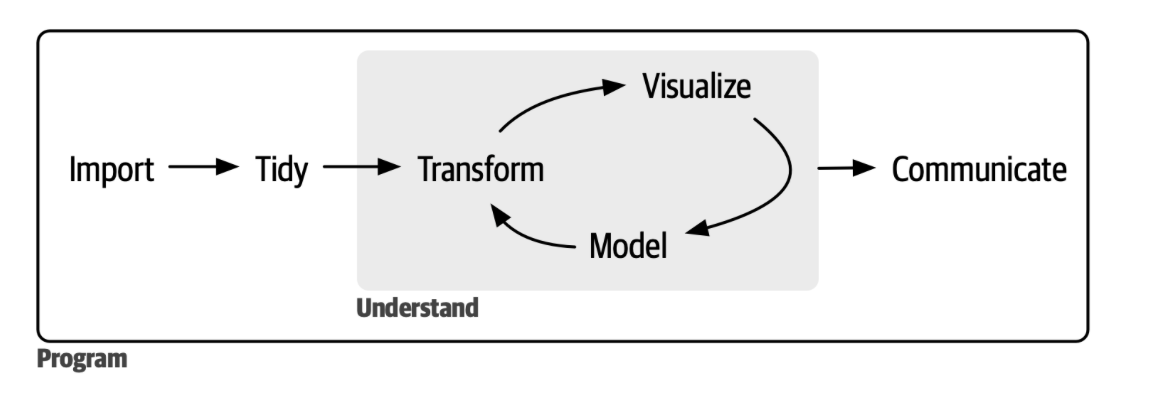
\includegraphics[width=0.8\linewidth,height=\textheight,keepaspectratio]{images/lec01_slide11_a.png}

\subsection{Today}\label{today}

\begin{itemize}
\tightlist
\item
  \textbf{Importing data}
\item
  \textbf{Merging datasets}
\item
  \textbf{Descriptive statistics:} grouping and summarizing data
\item
  \textbf{Exploratory data analysis}
\item
  \textbf{Survey data:} handling missing values and survey weights
\item
  \textbf{Making tables}
\end{itemize}

\subsection{Importing data in R}\label{importing-data-in-r}

\begin{itemize}
\tightlist
\item
  \textbf{Importing data} is usually the first step in any analysis
\item
  Different data formats require different packages
\item
  Most functions return a data frame
\item
  The same downstream tools (filter, mutate) etc work regardless of
  initial format
\item
  These import functions:

  \begin{itemize}
  \tightlist
  \item
    Read values into R
  \item
    Assign data types (numeric, character, factor, date etc)
  \item
    Recognise common missing value codes automatically and code them as
    NA
  \end{itemize}
\end{itemize}

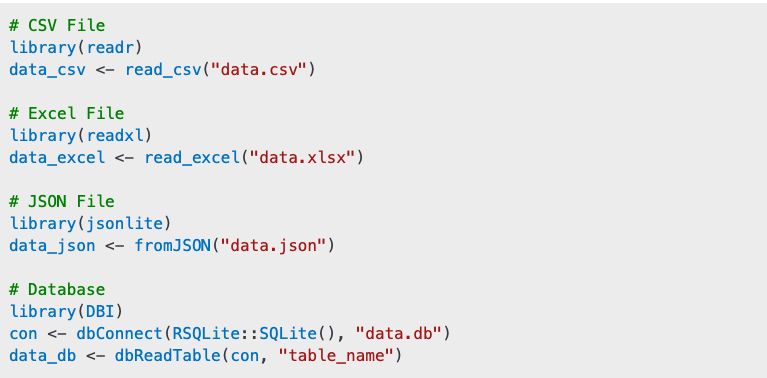
\includegraphics[width=1\linewidth,height=\textheight,keepaspectratio]{images/lec03_slide12_a.png}

\section{Merging Datasets}\label{merging-datasets}

\subsection{Merging dataframes}\label{merging-dataframes}

\begin{itemize}
\tightlist
\item
  To answer many real world questions, you often need to combine
  information from multiple datasets
\item
  To join two data frames you need:

  \begin{itemize}
  \tightlist
  \item
    Two data frames containing related information
  \item
    A key variable that appears in both data frames used to match rows
    across datasets
  \item
    A join function that tells R how to combine the data
  \end{itemize}
\end{itemize}

\subsection{Joins example}\label{joins-example}

\begin{itemize}
\tightlist
\item
  How do we combine information from two tables?
\end{itemize}

\begin{Shaded}
\begin{Highlighting}[]
\NormalTok{dogs }\OtherTok{\textless{}{-}} \FunctionTok{data.frame}\NormalTok{(}
  \AttributeTok{dog\_id =} \DecValTok{1}\SpecialCharTok{:}\DecValTok{4}\NormalTok{,}
  \AttributeTok{dog\_name =} \FunctionTok{c}\NormalTok{(}\StringTok{"Rover"}\NormalTok{, }\StringTok{"Fido"}\NormalTok{, }\StringTok{"Daisy"}\NormalTok{, }\StringTok{"Buddy"}\NormalTok{),}
  \AttributeTok{breed =} \FunctionTok{c}\NormalTok{(}\StringTok{"Great Dane"}\NormalTok{, }\StringTok{"Dalmatian"}\NormalTok{, }\StringTok{"Mutt"}\NormalTok{, }\StringTok{"Poodle"}\NormalTok{)}
\NormalTok{)}

\NormalTok{owners }\OtherTok{\textless{}{-}} \FunctionTok{data.frame}\NormalTok{(}
  \AttributeTok{owner\_id =} \DecValTok{1}\SpecialCharTok{:}\DecValTok{4}\NormalTok{,}
  \AttributeTok{owner\_name =} \FunctionTok{c}\NormalTok{(}\StringTok{"Alex"}\NormalTok{, }\StringTok{"Brenda"}\NormalTok{, }\StringTok{"Charlie"}\NormalTok{, }\StringTok{"Diana"}\NormalTok{),}
  \AttributeTok{dog\_name =} \FunctionTok{c}\NormalTok{(}\StringTok{"Buddy"}\NormalTok{, }\StringTok{"Artemis"}\NormalTok{, }\StringTok{"Fido"}\NormalTok{, }\StringTok{"Roger"}\NormalTok{)}
\NormalTok{)}

\NormalTok{dogs}
\end{Highlighting}
\end{Shaded}

\begin{verbatim}
  dog_id dog_name      breed
1      1    Rover Great Dane
2      2     Fido  Dalmatian
3      3    Daisy       Mutt
4      4    Buddy     Poodle
\end{verbatim}

\begin{Shaded}
\begin{Highlighting}[]
\NormalTok{owners}
\end{Highlighting}
\end{Shaded}

\begin{verbatim}
  owner_id owner_name dog_name
1        1       Alex    Buddy
2        2     Brenda  Artemis
3        3    Charlie     Fido
4        4      Diana    Roger
\end{verbatim}

What is the key variable? A key does not have to be numeric! But often
it is easy to have a numeric key. Especially for large datasets, can
make join quicker.

\subsection{Left join}\label{left-join}

\begin{itemize}
\tightlist
\item
  \texttt{left\_join(x,y)} keeps all observations in x, and matches as
  many rows in y as possible
\item
  Every row of x is preserved in the output
\item
  If there is no matching row in y, then it artificially creates an NA
  row in y to match with and puts it in the end
\end{itemize}

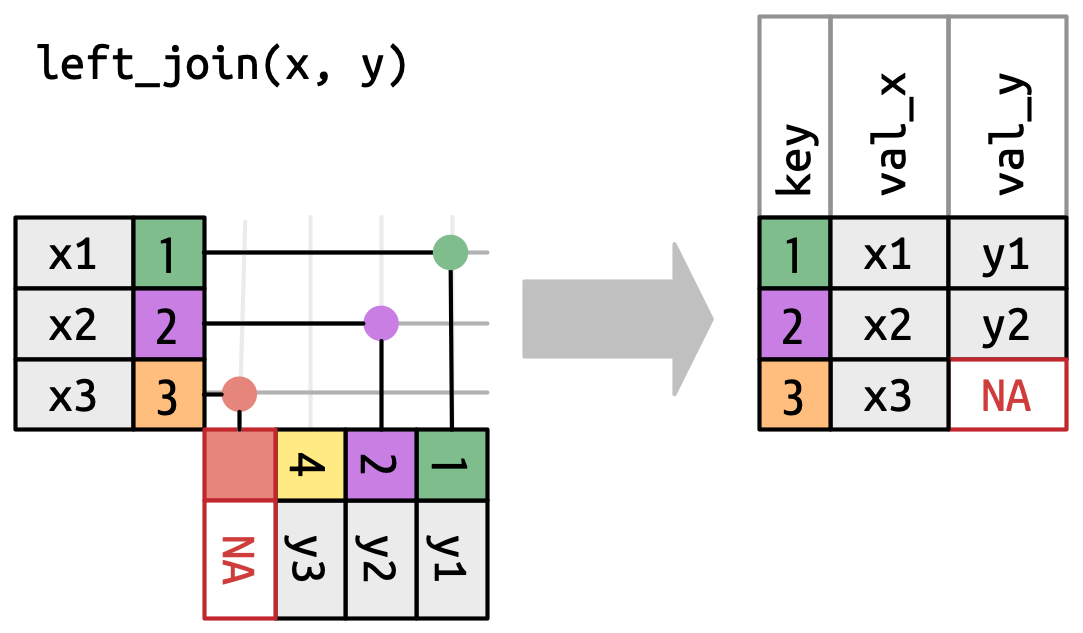
\includegraphics[width=1\linewidth,height=\textheight,keepaspectratio]{images/lec03_slide16_a.png}

\begin{Shaded}
\begin{Highlighting}[]
\NormalTok{owners }\SpecialCharTok{\%\textgreater{}\%} \FunctionTok{left\_join}\NormalTok{(dogs, }\AttributeTok{by =} \StringTok{"dog\_name"}\NormalTok{)}
\end{Highlighting}
\end{Shaded}

\begin{verbatim}
  owner_id owner_name dog_name dog_id     breed
1        1       Alex    Buddy      4    Poodle
2        2     Brenda  Artemis     NA      <NA>
3        3    Charlie     Fido      2 Dalmatian
4        4      Diana    Roger     NA      <NA>
\end{verbatim}

\subsection{Right join}\label{right-join}

\begin{itemize}
\tightlist
\item
  \texttt{right\_join(x,y)} keeps all observations in y and matches as
  many rows in x as possible
\item
  Every row of y is preserved in the output
\item
  If there is no matching row in x, then it artificially creates an NA
  row in x to match with and puts it in the end
\end{itemize}

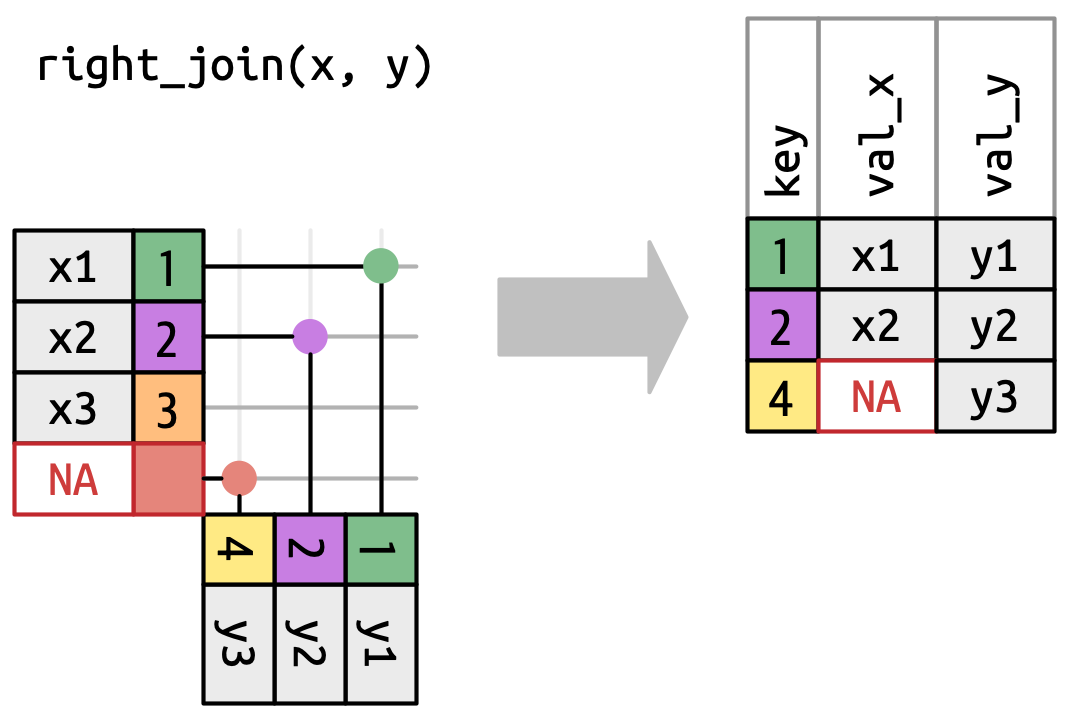
\includegraphics[width=1\linewidth,height=\textheight,keepaspectratio]{images/lec03_slide18_a.png}

\begin{Shaded}
\begin{Highlighting}[]
\NormalTok{owners }\SpecialCharTok{\%\textgreater{}\%} \FunctionTok{right\_join}\NormalTok{(dogs, }\AttributeTok{by =} \StringTok{"dog\_name"}\NormalTok{)}
\end{Highlighting}
\end{Shaded}

\begin{verbatim}
  owner_id owner_name dog_name dog_id      breed
1        1       Alex    Buddy      4     Poodle
2        3    Charlie     Fido      2  Dalmatian
3       NA       <NA>    Rover      1 Great Dane
4       NA       <NA>    Daisy      3       Mutt
\end{verbatim}

\subsection{Inner join}\label{inner-join}

\begin{itemize}
\tightlist
\item
  \texttt{inner\_join(x,y)} retains rows if and only if the keys are
  equal
\end{itemize}

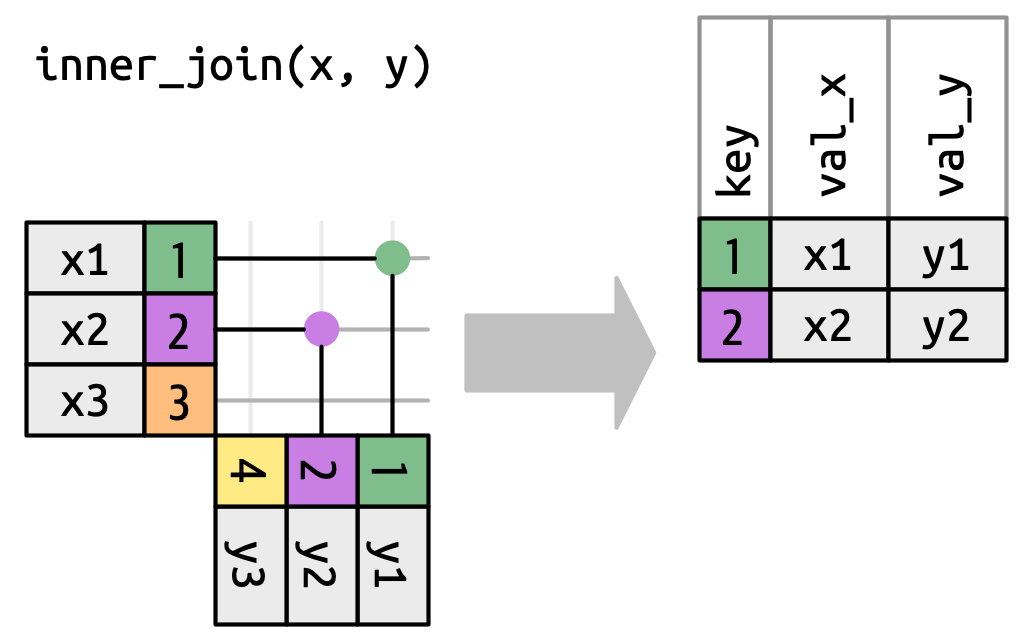
\includegraphics[width=1\linewidth,height=\textheight,keepaspectratio]{images/lec03_slide20_a.png}

\begin{Shaded}
\begin{Highlighting}[]
\NormalTok{owners }\SpecialCharTok{\%\textgreater{}\%} \FunctionTok{inner\_join}\NormalTok{(dogs, }\AttributeTok{by =} \StringTok{"dog\_name"}\NormalTok{)}
\end{Highlighting}
\end{Shaded}

\begin{verbatim}
  owner_id owner_name dog_name dog_id     breed
1        1       Alex    Buddy      4    Poodle
2        3    Charlie     Fido      2 Dalmatian
\end{verbatim}

\subsection{Full join}\label{full-join}

\begin{itemize}
\tightlist
\item
  \texttt{full\_join(x,y)} keeps all observations that appear in x or y
\item
  Every row of x and y is included in the output because both x and y
  have a fall back row of NAs
\item
  The output starts with all rows from x, followed by the remaining
  unmatched y rows
\end{itemize}

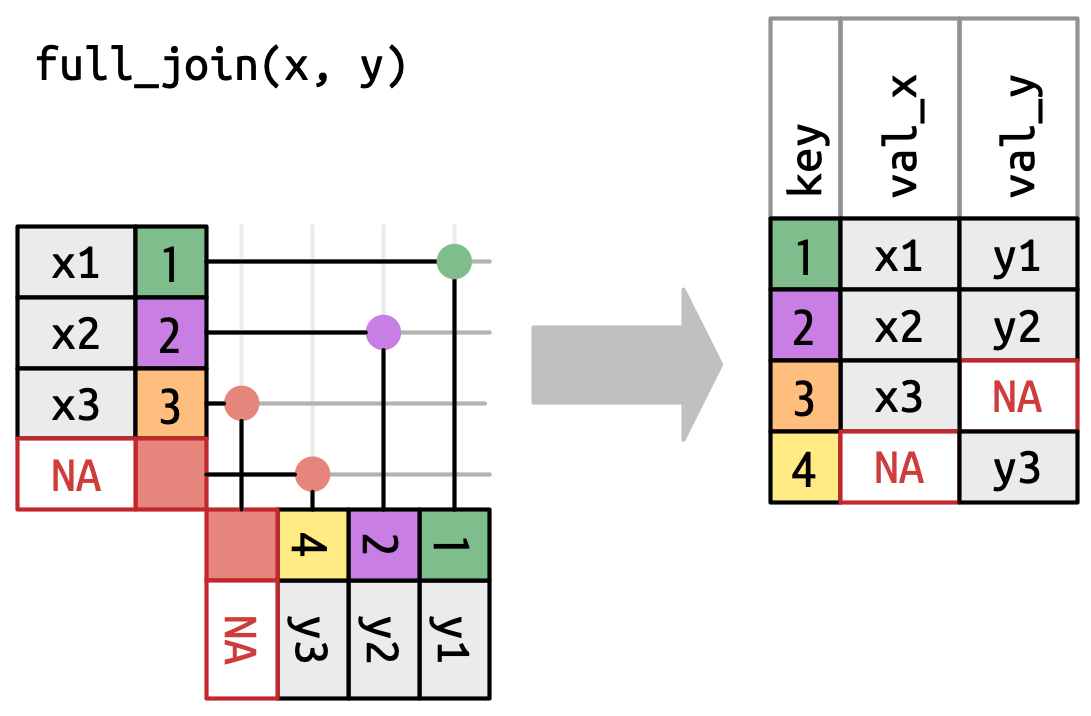
\includegraphics[width=1\linewidth,height=\textheight,keepaspectratio]{images/lec03_slide22_a.png}

\begin{Shaded}
\begin{Highlighting}[]
\NormalTok{owners }\SpecialCharTok{\%\textgreater{}\%} \FunctionTok{full\_join}\NormalTok{(dogs, }\AttributeTok{by =} \StringTok{"dog\_name"}\NormalTok{)}
\end{Highlighting}
\end{Shaded}

\begin{verbatim}
  owner_id owner_name dog_name dog_id      breed
1        1       Alex    Buddy      4     Poodle
2        2     Brenda  Artemis     NA       <NA>
3        3    Charlie     Fido      2  Dalmatian
4        4      Diana    Roger     NA       <NA>
5       NA       <NA>    Rover      1 Great Dane
6       NA       <NA>    Daisy      3       Mutt
\end{verbatim}

\subsection{Join types summary}\label{join-types-summary}


\includegraphics[width=0.8\linewidth,height=\textheight,keepaspectratio]{images/lec03_slide25_a.tiff}

\subsection{Key considerations for
merging}\label{key-considerations-for-merging}

\begin{itemize}
\tightlist
\item
  \textbf{Join does not require 1:1 matching}
\item
  If one owner matches multiple dogs, the owner's row will be repeated
  once for each match
\item
  \texttt{left\_join()} is the one you will use most often: allows you
  to add new variables onto your analysis dataframe
\end{itemize}

\subsection{When do joins increase the row
count?}\label{when-do-joins-increase-the-row-count}

\begin{Shaded}
\begin{Highlighting}[]
\CommentTok{\# When one owner has multiple dogs}
\NormalTok{owners\_v2 }\OtherTok{\textless{}{-}} \FunctionTok{data.frame}\NormalTok{(}
  \AttributeTok{owner\_id =} \DecValTok{1}\SpecialCharTok{:}\DecValTok{2}\NormalTok{,}
  \AttributeTok{owner\_name =} \FunctionTok{c}\NormalTok{(}\StringTok{"Alex"}\NormalTok{, }\StringTok{"Brenda"}\NormalTok{)}
\NormalTok{)}

\NormalTok{dogs\_v2 }\OtherTok{\textless{}{-}} \FunctionTok{data.frame}\NormalTok{(}
  \AttributeTok{dog\_id =} \DecValTok{1}\SpecialCharTok{:}\DecValTok{4}\NormalTok{,}
  \AttributeTok{owner\_id =} \FunctionTok{c}\NormalTok{(}\DecValTok{1}\NormalTok{, }\DecValTok{1}\NormalTok{, }\DecValTok{1}\NormalTok{, }\DecValTok{2}\NormalTok{),}
  \AttributeTok{dog\_name =} \FunctionTok{c}\NormalTok{(}\StringTok{"Rover"}\NormalTok{, }\StringTok{"Fido"}\NormalTok{, }\StringTok{"Daisy"}\NormalTok{, }\StringTok{"Buddy"}\NormalTok{),}
  \AttributeTok{breed =} \FunctionTok{c}\NormalTok{(}\StringTok{"Great Dane"}\NormalTok{, }\StringTok{"Dalmatian"}\NormalTok{, }\StringTok{"Mutt"}\NormalTok{, }\StringTok{"Poodle"}\NormalTok{)}
\NormalTok{)}

\NormalTok{owners\_v2 }\SpecialCharTok{\%\textgreater{}\%} \FunctionTok{left\_join}\NormalTok{(dogs\_v2, }\AttributeTok{by =} \StringTok{"owner\_id"}\NormalTok{)}
\end{Highlighting}
\end{Shaded}

\begin{verbatim}
  owner_id owner_name dog_id dog_name      breed
1        1       Alex      1    Rover Great Dane
2        1       Alex      2     Fido  Dalmatian
3        1       Alex      3    Daisy       Mutt
4        2     Brenda      4    Buddy     Poodle
\end{verbatim}

\subsection{Appending datasets with
bind\_rows()}\label{appending-datasets-with-bind_rows}

\begin{itemize}
\tightlist
\item
  \texttt{bind\_rows()} appends dataframes row-wise
\item
  Requires the same column names
\item
  Missing columns are filled with NAs
\item
  Mental model: ``put these datasets underneath each other''
\end{itemize}

\begin{Shaded}
\begin{Highlighting}[]
\NormalTok{df1 }\OtherTok{\textless{}{-}} \FunctionTok{data.frame}\NormalTok{(}\AttributeTok{x =} \DecValTok{1}\SpecialCharTok{:}\DecValTok{3}\NormalTok{, }\AttributeTok{y =} \FunctionTok{c}\NormalTok{(}\StringTok{"a"}\NormalTok{, }\StringTok{"b"}\NormalTok{, }\StringTok{"c"}\NormalTok{))}
\NormalTok{df2 }\OtherTok{\textless{}{-}} \FunctionTok{data.frame}\NormalTok{(}\AttributeTok{x =} \DecValTok{4}\SpecialCharTok{:}\DecValTok{5}\NormalTok{, }\AttributeTok{y =} \FunctionTok{c}\NormalTok{(}\StringTok{"d"}\NormalTok{, }\StringTok{"e"}\NormalTok{))}

\NormalTok{df1 }\SpecialCharTok{\%\textgreater{}\%} \FunctionTok{bind\_rows}\NormalTok{(df2)}
\end{Highlighting}
\end{Shaded}

\begin{verbatim}
  x y
1 1 a
2 2 b
3 3 c
4 4 d
5 5 e
\end{verbatim}

\section{Descriptive Statistics: Grouping and Summarizing
Data}\label{descriptive-statistics-grouping-and-summarizing-data}

\subsection{Functions we've covered so
far}\label{functions-weve-covered-so-far}

\begin{itemize}
\tightlist
\item
  \textbf{\texttt{filter()}} - select rows based on conditions
\item
  \textbf{\texttt{select()}} - choose columns
\item
  \textbf{\texttt{mutate()}} - create new variables
\item
  \textbf{\texttt{arrange()}} - sort rows
\end{itemize}

\subsection{Converting between different variable
types}\label{converting-between-different-variable-types}

\begin{itemize}
\tightlist
\item
  Find out how your variable is stored using \texttt{class(df\$varname)}
\item
  Variable types:

  \begin{itemize}
  \tightlist
  \item
    \textbf{Numeric:} for calculations
  \item
    \textbf{Factor:} categorical variable with levels
  \item
    \textbf{Character:} text strings
  \item
    \textbf{Date:} temporal data
  \item
    \textbf{Logical:} TRUE/FALSE
  \end{itemize}
\item
  Different classes behave very differently in models and plots --- the
  same variable (e.g.~year) may be treated as:

  \begin{itemize}
  \tightlist
  \item
    \textbf{Numeric} → trends, slopes, extrapolation
  \item
    \textbf{Factor} → group comparisons, year fixed effects
  \end{itemize}
\item
  R stores factor variables as a set of labels stuck onto numbered boxes
\end{itemize}

\subsection{Converting between variable types in
R}\label{converting-between-variable-types-in-r}

\begin{itemize}
\tightlist
\item
  Convert year variable stored as numeric to factor:
\end{itemize}

\begin{Shaded}
\begin{Highlighting}[]
\NormalTok{df }\OtherTok{\textless{}{-}}\NormalTok{ df }\SpecialCharTok{\%\textgreater{}\%} \FunctionTok{mutate}\NormalTok{(}\AttributeTok{year\_f =} \FunctionTok{as.factor}\NormalTok{(year))}
\end{Highlighting}
\end{Shaded}

\begin{itemize}
\tightlist
\item
  Convert year variable stored as factor to numeric:
\end{itemize}

\begin{Shaded}
\begin{Highlighting}[]
\NormalTok{df }\OtherTok{\textless{}{-}}\NormalTok{ df }\SpecialCharTok{\%\textgreater{}\%} \FunctionTok{mutate}\NormalTok{(}\AttributeTok{year =} \FunctionTok{as.numeric}\NormalTok{(}\FunctionTok{as.character}\NormalTok{(year\_f)))}
\end{Highlighting}
\end{Shaded}

\begin{itemize}
\tightlist
\item
  \texttt{as.character} converts to a string containing the labels,
  which can then be converted to a factor
\end{itemize}

\subsection{case\_when()}\label{case_when}

\begin{itemize}
\tightlist
\item
  \texttt{case\_when} applies a series of if-else rules from top to
  bottom
\item
  Useful for defining categorical variables based on existing variables
\item
  \texttt{between} checks whether a numeric value lies between two
  values
\end{itemize}

\begin{Shaded}
\begin{Highlighting}[]
\NormalTok{df }\OtherTok{\textless{}{-}}\NormalTok{ df }\SpecialCharTok{\%\textgreater{}\%}
  \FunctionTok{mutate}\NormalTok{(}
    \AttributeTok{age\_group =} \FunctionTok{case\_when}\NormalTok{(}
      \FunctionTok{between}\NormalTok{(age, }\DecValTok{0}\NormalTok{, }\DecValTok{17}\NormalTok{)  }\SpecialCharTok{\textasciitilde{}} \StringTok{"Child"}\NormalTok{,}
      \FunctionTok{between}\NormalTok{(age, }\DecValTok{18}\NormalTok{, }\DecValTok{39}\NormalTok{) }\SpecialCharTok{\textasciitilde{}} \StringTok{"Young adult"}\NormalTok{,}
      \FunctionTok{between}\NormalTok{(age, }\DecValTok{40}\NormalTok{, }\DecValTok{64}\NormalTok{) }\SpecialCharTok{\textasciitilde{}} \StringTok{"Middle{-}aged"}\NormalTok{,}
\NormalTok{      age }\SpecialCharTok{\textgreater{}=} \DecValTok{65}            \SpecialCharTok{\textasciitilde{}} \StringTok{"Older adult"}\NormalTok{,}
      \ConstantTok{TRUE}                 \SpecialCharTok{\textasciitilde{}} \ConstantTok{NA\_character\_}
\NormalTok{    )}
\NormalTok{  )}
\end{Highlighting}
\end{Shaded}

\subsection{summarise()}\label{summarise}

\begin{itemize}
\tightlist
\item
  \texttt{summarise()} reduces a dataset to one or more summary values
\item
  Each summary is computed over all rows in the data
\item
  Common summaries include: mean, standard deviation, sum, count
\item
  Can compute many summary stats at the same time
\item
  If applied to the whole dataframe without grouping, will return a
  one-row dataset containing the summary stats
\item
  Many summary functions return NA if any values are missing. Use
  \texttt{na.rm=TRUE} if you don't want this
\end{itemize}

\begin{Shaded}
\begin{Highlighting}[]
\NormalTok{df }\SpecialCharTok{\%\textgreater{}\%}
  \FunctionTok{summarise}\NormalTok{(}
    \AttributeTok{mean\_var1 =} \FunctionTok{mean}\NormalTok{(var1, }\AttributeTok{na.rm =} \ConstantTok{TRUE}\NormalTok{),}
    \AttributeTok{n =} \FunctionTok{n}\NormalTok{()}
\NormalTok{  )}
\end{Highlighting}
\end{Shaded}

\subsection{group\_by()}\label{group_by}

\begin{itemize}
\tightlist
\item
  \texttt{group\_by()} allows you to group a data frame by one or more
  categorical variable
\item
  It does not change the data but changes how later functions behave:
  ``From now on, do things separately for each group''
\item
  Commonly used before \texttt{summarise()} to produce summary
  statistics by group
\item
  Suppose \texttt{var2} is a categorical variable that takes three
  distinct values --- what will this code produce?
\end{itemize}

\begin{Shaded}
\begin{Highlighting}[]
\NormalTok{df }\SpecialCharTok{\%\textgreater{}\%}
  \FunctionTok{group\_by}\NormalTok{(var2) }\SpecialCharTok{\%\textgreater{}\%}
  \FunctionTok{summarise}\NormalTok{(}
    \AttributeTok{mean\_var1 =} \FunctionTok{mean}\NormalTok{(var1, }\AttributeTok{na.rm =} \ConstantTok{TRUE}\NormalTok{),}
    \AttributeTok{n =} \FunctionTok{n}\NormalTok{()}
\NormalTok{  )}
\end{Highlighting}
\end{Shaded}

\subsection{ungroup()}\label{ungroup}

\begin{itemize}
\tightlist
\item
  Good practice to add \texttt{ungroup()} after grouping so you retrieve
  the original data frame
\item
  Stops you accidentally applying future operations to grouped data
\item
  Can also add \texttt{groups\ =\ "drop"} inside \texttt{summarise}
\end{itemize}

\begin{Shaded}
\begin{Highlighting}[]
\NormalTok{df }\SpecialCharTok{\%\textgreater{}\%}
  \FunctionTok{group\_by}\NormalTok{(var2) }\SpecialCharTok{\%\textgreater{}\%}
  \FunctionTok{summarise}\NormalTok{(}
    \AttributeTok{mean\_var1 =} \FunctionTok{mean}\NormalTok{(var1, }\AttributeTok{na.rm =} \ConstantTok{TRUE}\NormalTok{),}
    \AttributeTok{n =} \FunctionTok{n}\NormalTok{()}
\NormalTok{  ) }\SpecialCharTok{\%\textgreater{}\%}
  \FunctionTok{ungroup}\NormalTok{()}
\end{Highlighting}
\end{Shaded}

\subsection{Check your understanding}\label{check-your-understanding}

\begin{itemize}
\tightlist
\item
  Suppose we have the following data frame:
\end{itemize}

\begin{Shaded}
\begin{Highlighting}[]
\NormalTok{df }\OtherTok{\textless{}{-}} \FunctionTok{data.frame}\NormalTok{(}
     \AttributeTok{x =} \DecValTok{1}\SpecialCharTok{:}\DecValTok{5}\NormalTok{,}
     \AttributeTok{y =} \FunctionTok{c}\NormalTok{(}\StringTok{"a"}\NormalTok{, }\StringTok{"b"}\NormalTok{, }\StringTok{"a"}\NormalTok{, }\StringTok{"a"}\NormalTok{, }\StringTok{"b"}\NormalTok{),}
     \AttributeTok{z =} \FunctionTok{c}\NormalTok{(}\StringTok{"K"}\NormalTok{, }\StringTok{"K"}\NormalTok{, }\StringTok{"L"}\NormalTok{, }\StringTok{"L"}\NormalTok{, }\StringTok{"K"}\NormalTok{)}
\NormalTok{)}

\NormalTok{df}
\end{Highlighting}
\end{Shaded}

\begin{verbatim}
  x y z
1 1 a K
2 2 b K
3 3 a L
4 4 a L
5 5 b K
\end{verbatim}

\begin{itemize}
\tightlist
\item
  What would the following code do? (Don't run the code! Think about
  what the output may look like)
\end{itemize}

\begin{Shaded}
\begin{Highlighting}[]
\NormalTok{df }\SpecialCharTok{\%\textgreater{}\%} \FunctionTok{group\_by}\NormalTok{(y)}
\end{Highlighting}
\end{Shaded}

\begin{verbatim}
# A tibble: 5 × 3
# Groups:   y [2]
      x y     z
  <int> <chr> <chr>
1     1 a     K
2     2 b     K
3     3 a     L
4     4 a     L
5     5 b     K
\end{verbatim}

\subsection{Check your understanding}\label{check-your-understanding-1}

\begin{itemize}
\tightlist
\item
  What would the following code do?
\end{itemize}

\begin{Shaded}
\begin{Highlighting}[]
\NormalTok{df }\SpecialCharTok{\%\textgreater{}\%} \FunctionTok{arrange}\NormalTok{(y)}
\end{Highlighting}
\end{Shaded}

\subsection{Check your understanding}\label{check-your-understanding-2}

\begin{itemize}
\tightlist
\item
  What would the following code do?
\end{itemize}

\begin{Shaded}
\begin{Highlighting}[]
\NormalTok{df }\SpecialCharTok{\%\textgreater{}\%}
  \FunctionTok{group\_by}\NormalTok{(y) }\SpecialCharTok{\%\textgreater{}\%}
  \FunctionTok{summarize}\NormalTok{(}\AttributeTok{mean\_x =} \FunctionTok{mean}\NormalTok{(x))}
\end{Highlighting}
\end{Shaded}

\begin{verbatim}
# A tibble: 2 × 2
  y     mean_x
  <chr>  <dbl>
1 a       2.67
2 b       3.5
\end{verbatim}

\subsection{Check your understanding}\label{check-your-understanding-3}

\begin{itemize}
\tightlist
\item
  What would the following code do?
\end{itemize}

\begin{Shaded}
\begin{Highlighting}[]
\NormalTok{df }\SpecialCharTok{\%\textgreater{}\%}
  \FunctionTok{group\_by}\NormalTok{(y, z) }\SpecialCharTok{\%\textgreater{}\%}
  \FunctionTok{summarize}\NormalTok{(}\AttributeTok{mean\_x =} \FunctionTok{mean}\NormalTok{(x))}
\end{Highlighting}
\end{Shaded}

\begin{verbatim}
# A tibble: 3 × 3
# Groups:   y [2]
  y     z     mean_x
  <chr> <chr>  <dbl>
1 a     K        1
2 a     L        3.5
3 b     K        3.5
\end{verbatim}

\subsection{Check your understanding}\label{check-your-understanding-4}

\begin{itemize}
\tightlist
\item
  What would the following code do?
\end{itemize}

\begin{Shaded}
\begin{Highlighting}[]
\NormalTok{df }\SpecialCharTok{\%\textgreater{}\%}
  \FunctionTok{group\_by}\NormalTok{(y, z) }\SpecialCharTok{\%\textgreater{}\%}
  \FunctionTok{mutate}\NormalTok{(}\AttributeTok{mean\_x =} \FunctionTok{mean}\NormalTok{(x))}
\end{Highlighting}
\end{Shaded}

\begin{verbatim}
# A tibble: 5 × 4
# Groups:   y, z [3]
      x y     z     mean_x
  <int> <chr> <chr>  <dbl>
1     1 a     K        1
2     2 b     K        3.5
3     3 a     L        3.5
4     4 a     L        3.5
5     5 b     K        3.5
\end{verbatim}

\section{Exploratory Data Analysis}\label{exploratory-data-analysis}

\subsection{What is EDA?}\label{what-is-eda}

\begin{itemize}
\tightlist
\item
  Exploratory Data Analysis (EDA) is the process of interrogating data
  in a systematic way to understand what it contains and how it was
  generated
\item
  It typically includes:

  \begin{itemize}
  \tightlist
  \item
    Examining distributions (levels, spread, outliers)
  \item
    Comparing groups and subpopulations to look for heterogeneity
  \item
    Visualising relationships between key variables
  \item
    Investigating missing data patterns
  \end{itemize}
\item
  \textbf{It is iterative:} findings from one step shape the next
  question
\end{itemize}

\subsection{Why Exploratory Data Analysis
matters}\label{why-exploratory-data-analysis-matters}

\begin{itemize}
\tightlist
\item
  EDA sits between data wrangling and modelling in the analytics
  pipeline:

  \begin{itemize}
  \tightlist
  \item
    \textbf{Wrangling:} get the data into usable form
  \item
    \textbf{EDA:} understand what you actually have
  \item
    \textbf{Modelling:} answer a specific question under assumptions
  \end{itemize}
\item
  EDA helps you:

  \begin{itemize}
  \tightlist
  \item
    Detect data errors, coding problems and inconsistencies
  \item
    Understand sample selection and missingness
  \item
    Identify relevant variation, correlation between variables and
    heterogeneity
  \item
    Decide which analyses are credible and which are not
  \end{itemize}
\item
  \textbf{If you do not understand your data, no model can save you!}
\end{itemize}

\section{Survey data}\label{survey-data}

\subsection{Survey weights}\label{survey-weights}

\begin{itemize}
\tightlist
\item
  Adjustments applied to survey data to ensure that results represent
  the target population
\item
  \textbf{Reasons for using survey weights:}

  \begin{itemize}
  \tightlist
  \item
    \textbf{Unequal Sampling Probabilities:} Some groups are
    intentionally oversampled (e.g., racial minorities, elderly, rural
    residence) to ensure sufficient sample size
  \item
    \textbf{Nonresponse:} To account for differences between those who
    responded and those who didn't
  \item
    \textbf{Post-stratification adjustment:} Aligns survey data with
    known population distributions (e.g., age, gender)
  \end{itemize}
\item
  \textbf{Core idea:} each observation in the sample represents itself
  plus others in the population

  \begin{itemize}
  \tightlist
  \item
    ``Analysis weights'' are scaled to sum to the sample size
  \item
    ``Population weights'' are scaled to sum to the population size
  \end{itemize}
\end{itemize}

\subsection{Using survey weights in R}\label{using-survey-weights-in-r}

\begin{itemize}
\tightlist
\item
  \textbf{Core R packages:}

  \begin{itemize}
  \tightlist
  \item
    \texttt{survey} and \texttt{srvyr} packages
  \item
    \texttt{srvyr} integrates well with tidyverse for a user-friendly
    workflow
  \end{itemize}
\item
  \textbf{Key Steps:}

  \begin{enumerate}
  \def\labelenumi{\arabic{enumi}.}
  \tightlist
  \item
    Load libraries!
  \item
    Load survey data
  \item
    Define the survey design using weights
  \item
    Use design for analysis
  \item
    READ the manual
  \end{enumerate}
\item
  IPUMS has detailed description of weights for each data series and
  code snippets explaining how to work with them
\end{itemize}

\subsection{Survey weights: Important
caveat}\label{survey-weights-important-caveat}

\begin{itemize}
\tightlist
\item
  You can calculate many summary statistics by applying weights manually
  (e.g.~\texttt{weighted.mean()})
\item
  However, standard errors can get very complicated so it's usually
  better to work with the designed survey approach
\item
  \textbf{CAUTION:} must make sure you use the functions designed for
  survey analysis

  \begin{itemize}
  \tightlist
  \item
    \texttt{survey\_mean()} not \texttt{mean()}
  \item
    \texttt{survey\_total()} not \texttt{n()}
  \end{itemize}
\item
  Most regular functions will not throw an error!
\end{itemize}

\subsection{Survey weights example}\label{survey-weights-example}

\begin{Shaded}
\begin{Highlighting}[]
\CommentTok{\# Install if needed: install.packages(c("survey", "srvyr"))}
\FunctionTok{library}\NormalTok{(survey)}
\FunctionTok{library}\NormalTok{(srvyr)}

\CommentTok{\# Create example survey data}
\FunctionTok{set.seed}\NormalTok{(}\DecValTok{123}\NormalTok{)}
\NormalTok{survey\_data }\OtherTok{\textless{}{-}} \FunctionTok{tibble}\NormalTok{(}
  \AttributeTok{id =} \DecValTok{1}\SpecialCharTok{:}\DecValTok{100}\NormalTok{,}
  \AttributeTok{outcome =} \FunctionTok{rnorm}\NormalTok{(}\DecValTok{100}\NormalTok{, }\AttributeTok{mean =} \DecValTok{50}\NormalTok{, }\AttributeTok{sd =} \DecValTok{10}\NormalTok{),}
  \AttributeTok{weight =} \FunctionTok{rnorm}\NormalTok{(}\DecValTok{100}\NormalTok{, }\AttributeTok{mean =} \DecValTok{1}\NormalTok{, }\AttributeTok{sd =} \FloatTok{0.2}\NormalTok{),}
  \AttributeTok{stratum =} \FunctionTok{rep}\NormalTok{(}\FunctionTok{c}\NormalTok{(}\StringTok{"A"}\NormalTok{, }\StringTok{"B"}\NormalTok{), }\DecValTok{50}\NormalTok{)}
\NormalTok{)}

\CommentTok{\# Design survey with weights}
\NormalTok{survey\_design }\OtherTok{\textless{}{-}}\NormalTok{ survey\_data }\SpecialCharTok{\%\textgreater{}\%}
  \FunctionTok{as\_survey\_design}\NormalTok{(}\AttributeTok{ids =}\NormalTok{ id, }\AttributeTok{weights =}\NormalTok{ weight, }\AttributeTok{strata =}\NormalTok{ stratum)}

\CommentTok{\# Calculate weighted mean and confidence interval}
\NormalTok{survey\_design }\SpecialCharTok{\%\textgreater{}\%}
  \FunctionTok{summarise}\NormalTok{(}
    \AttributeTok{mean\_outcome =} \FunctionTok{survey\_mean}\NormalTok{(outcome, }\AttributeTok{na.rm =} \ConstantTok{TRUE}\NormalTok{),}
    \AttributeTok{total\_outcome =} \FunctionTok{survey\_total}\NormalTok{(outcome, }\AttributeTok{na.rm =} \ConstantTok{TRUE}\NormalTok{)}
\NormalTok{  )}
\end{Highlighting}
\end{Shaded}

\begin{verbatim}
# A tibble: 1 x 4
  mean_outcome mean_outcome_se total_outcome total_outcome_se
         <dbl>           <dbl>         <dbl>            <dbl>
1         50.8           0.908         4972.             127.
\end{verbatim}

\section{Missing data}\label{missing-data}

\subsection{Understanding missing
data}\label{understanding-missing-data}

\begin{itemize}
\tightlist
\item
  In R missing values are usually coded as \texttt{NA}

  \begin{itemize}
  \tightlist
  \item
    \texttt{sum(is.na())} counts the number of missing values
  \item
    To ignore missing values in analysis, we can filter them out with
    \texttt{filter(!is.na(var))} or ignore them for particular functions
    with \texttt{na.rm=TRUE}
  \end{itemize}
\item
  \textbf{Why might this be a problem?}

  \begin{itemize}
  \tightlist
  \item
    Dropping missing values is conditioning on being observed
  \item
    If missingness is related to outcomes or key variables, this can
    introduce bias
  \end{itemize}
\end{itemize}

\subsection{Types of missing data}\label{types-of-missing-data}

\begin{itemize}
\tightlist
\item
  Not all ``missing'' values mean the same thing:

  \begin{itemize}
  \tightlist
  \item
    \textbf{Not in universe (NIU):} respondent was not eligible / not
    asked
  \item
    \textbf{Refused:} respondent chose not to answer
  \item
    \textbf{Don't know / not ascertained}
  \end{itemize}
\item
  \textbf{Why this matters} --- these categories reflect different
  data-generating processes:

  \begin{itemize}
  \tightlist
  \item
    \textbf{NIU:} Usually safe to exclude from analysis by design ---
    these observations should not be treated as zero or ``no''
  \item
    \textbf{Refused:} People who refuse may systematically differ from
    those who answer
  \end{itemize}
\item
  \textbf{How you handle missing data is a substantive analysis
  decision, not just a coding choice!}
\end{itemize}

\subsection{Dealing with missing data}\label{dealing-with-missing-data}

\begin{itemize}
\tightlist
\item
  \textbf{Complete-case analysis (drop missing observations)}

  \begin{itemize}
  \tightlist
  \item
    Reasonable when missingness is plausibly unrelated to outcomes or
    key variables
  \item
    Risky when missingness reflects behaviour, health, or access
  \end{itemize}
\item
  \textbf{Recode missing categories explicitly}

  \begin{itemize}
  \tightlist
  \item
    Treat ``Refused'' or ``Don't know'' as their own categories
  \item
    Useful when missingness is informative
  \end{itemize}
\item
  \textbf{Imputation}

  \begin{itemize}
  \tightlist
  \item
    Replace missing values using information from other variables
  \item
    Requires assumptions about the missingness process
  \item
    Can reduce bias and improve precision (need to use multiple
    imputation to account for uncertainty)
  \end{itemize}
\item
  \textbf{Weighting adjustments (survey data)}

  \begin{itemize}
  \tightlist
  \item
    Adjust survey weights to account for differential non-response
  \item
    Often done by survey producers
  \item
    Relies on assumptions about who responds
  \end{itemize}
\end{itemize}

\subsection{A note on variable types}\label{a-note-on-variable-types}

\begin{itemize}
\tightlist
\item
  Factor variables from survey data are often saved in R as numeric
  data, or numeric data plus labels --- this can be convenient because
  you can use commands designed for numeric variables like
  \texttt{between()}
\item
  But you may need to convert to factor for some analyses:

  \begin{itemize}
  \tightlist
  \item
    Numeric encoding is convenient for quick filtering and comparisons
  \item
    But categorical operations (grouping, contrasts) need factors
  \item
    Always check your data structure with \texttt{str()} or
    \texttt{class()}
  \item
    Use \texttt{as.factor()} to convert when needed
  \end{itemize}
\end{itemize}

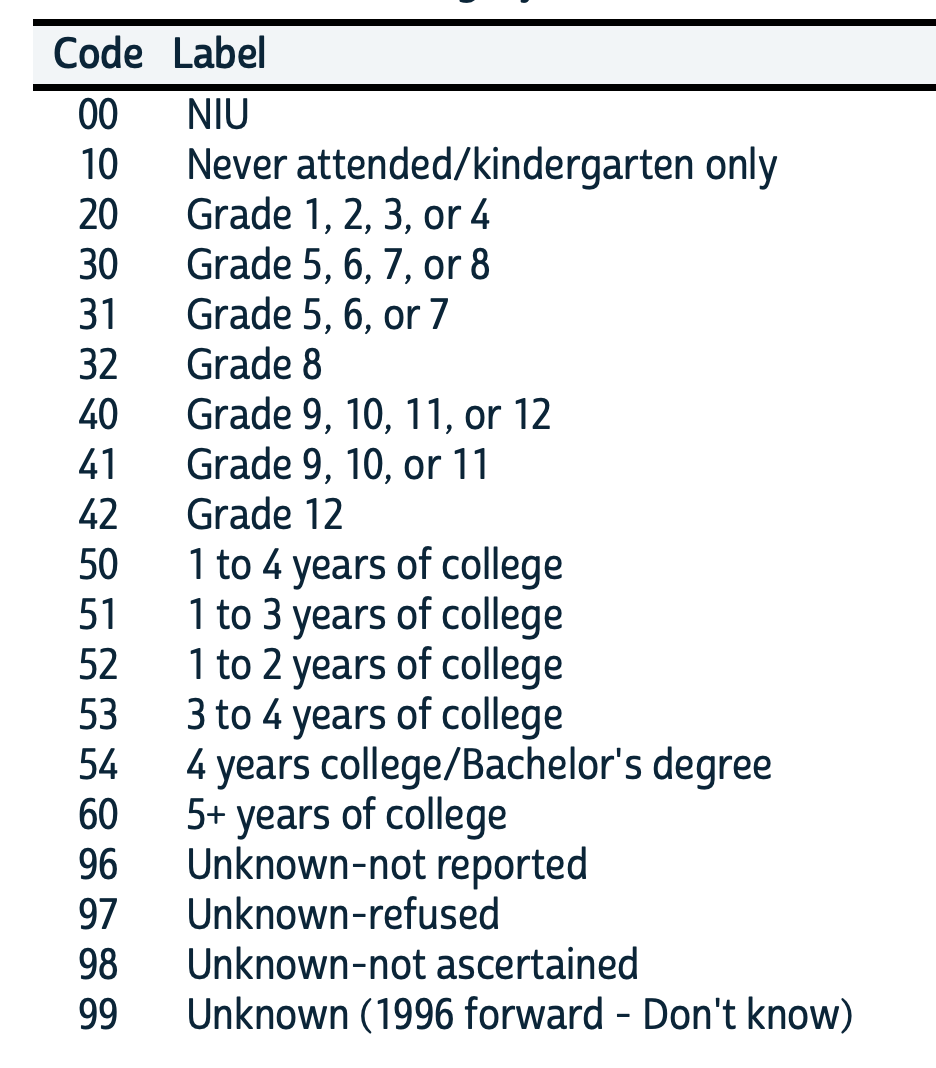
\includegraphics[width=1\linewidth,height=\textheight,keepaspectratio]{images/lec04_slide56_a.png}

\subsection{Making tables}\label{making-tables}

\begin{itemize}
\tightlist
\item
  Many packages for producing attractive tables in R
\item
  We will use \texttt{kableExtra} in this course
\item
  Two steps:

  \begin{enumerate}
  \def\labelenumi{\arabic{enumi}.}
  \tightlist
  \item
    Create a data frame with the quantities you want in the table
  \item
    Pipe it into the \texttt{kable} function to add styling!
  \end{enumerate}
\end{itemize}

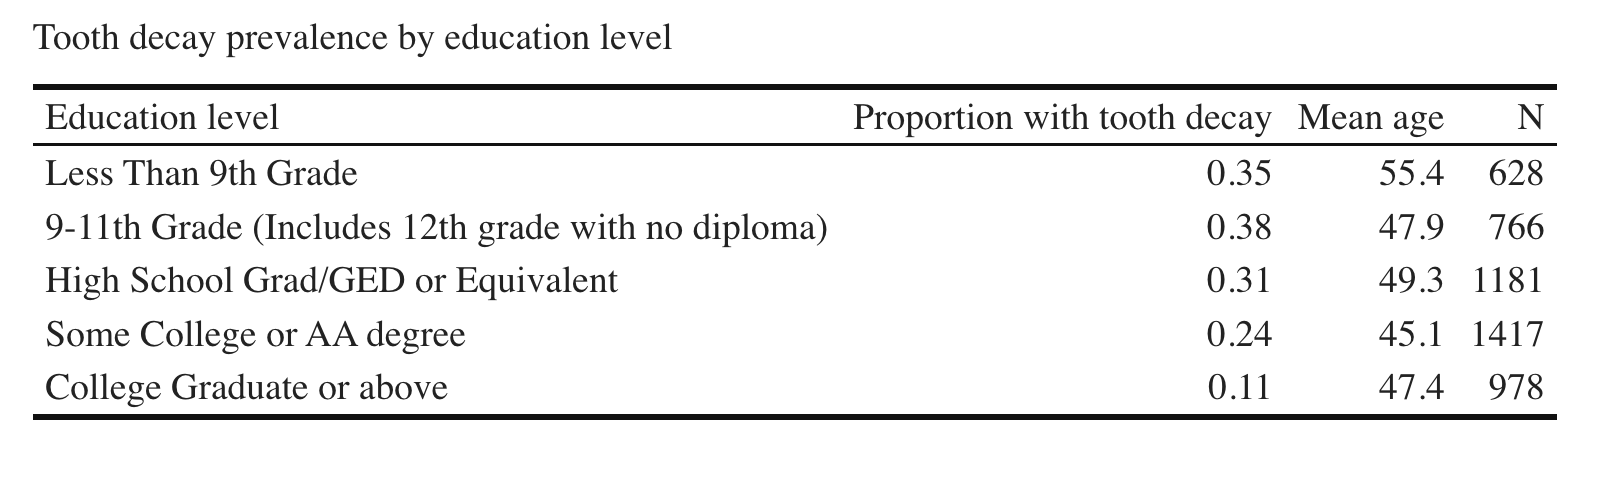
\includegraphics[width=0.6\linewidth,height=\textheight,keepaspectratio]{images/lec03_slide42_a.png}

\subsection{National Health and Nutrition Examination Survey
(NHANES)}\label{national-health-and-nutrition-examination-survey-nhanes}

\begin{itemize}
\tightlist
\item
  U.S. health survey that combines interviews, physical exams, and lab
  data to measure health, nutrition, and social determinants across the
  population
\item
  \textbf{Cross-sectional sample} taken every 2 years since 1999
  (\textasciitilde5,000 participants/round)
\item
  \textbf{Stratified, multi-stage sampling} with oversampling of key
  groups (e.g., racial/ethnic minorities, older adults)
\item
  \textbf{Good for:} estimating population prevalence (e.g., obesity,
  diabetes), comparing subgroups, and tracking trends
\item
  \textbf{Can be tricky to work with:}

  \begin{itemize}
  \tightlist
  \item
    Complex survey design ⇒ survey weights required
  \item
    Lots of missing data and complex ``skip patterns'' (rules about who
    gets asked what)
  \item
    Variable naming changes across cycles
  \end{itemize}
\item
  \textbf{R packages:} \texttt{nhanes} (first tutorial) and
  \texttt{nhanesA} (exercise)
\item
  These packages harmonise the underlying data and add codebooks to make
  it easier to work with
\end{itemize}


\includegraphics[width=1\linewidth,height=\textheight,keepaspectratio]{images/lec03_slide43_a.png}

\subsection{Takeaways}\label{takeaways}

\begin{itemize}
\tightlist
\item
  \textbf{Importing data:} first step is to get your data into a
  dataframe!
\item
  \textbf{Merging datasets:} \texttt{left\_join()} is the workhorse for
  adding variables to your analysis dataframe
\item
  \textbf{Summarising data:} \texttt{group\_by()} + \texttt{summarise()}
  to calculate descriptive statistics for subsets of your data
\item
  \textbf{Exploratory data analysis:} get a feel for your data by
  looking at distributions, group differences, and missingness
  \emph{before} modelling
\item
  \textbf{Survey data} is common in health analytics and needs to be
  handled carefully. Use survey weights via \texttt{survey} /
  \texttt{srvyr} (\texttt{survey\_mean()}, not \texttt{mean()})
\item
  \textbf{Take care with missing data:} always think about the process
  generating missing data
\end{itemize}




\end{document}
